\subsubsection{\stid{2.11} BOLT: Lightning Fast OpenMP}\label{subsubsect:bolt}

\paragraph{Overview}

OpenMP is central for several applications that target Exascale,
including ECP applications, to exploit on-node computational
resources.  Unfortunately, current production OpenMP runtimes, such as
those that ship with Intel and GNU compilers, are inadequate for the
massive and fine-grained concurrency expected at the Exascale level.
These runtimes rely on heavy-handed OS-level threading strategies that
incur significant overheads at fine-grained levels and exacerbate
interoperability issues between OpenMP and internode programming
systems, such as MPI and OpenSHMEM.  BOLT is a production quality
OpenMP runtime (called BOLT) which has been developed within the
SOLLVE project to address this issue by leveraging user-level threads
instead of OS-level threads (e.g., Pthreads).  Due to their
lightweight nature, managing and scheduling user-level threads incurs
significantly less overheads.  Furthermore, interoperability between
BOLT and internode programming systems opens up new optimization
opportunities by promoting asynchrony and reducing hardware
synchronization (atomics and memory barriers).  Initial studies on
this proposal can be found in \cite{amer2018, ccgrid, ppopp}. This
report briefly summarizes the issues in OpenMP runtimes that rely on
OS-level threading, describes BOLT as the solution to this challenge,
the current status in the BOLT effort, and the next steps for further
improvements.

\paragraph{Key Challenges}

The growing hardware concurrency in HPC
cluster nodes is pushing applications to chunk work more fine-grained
to expose parallelism opportunities.  This is often achieved through
nested parallelism either in the form of parallel regions or by
explicit tasks.  Nested parallel regions can potentially cause
oversubscription of OS-level threads to CPUs and thus lead to
expensive OS-level thread management.  Such heavy costs usually
outweigh the benefits of increased concurrency and thus compel the
OpenMP programmer to avoid nested parallel regions altogether.  Such
workaround, however, not only causes poor resource utilization from
insufficient parallelism but is also not always possible.  For
instance, the nested level could be outside the control of the user
because it belongs to an external library that also uses OpenMP
internally.  Internode programming systems, such as MPI and OpenSHMEM,
are not aware of OpenMP semantics, such as the notion of an OpenMP
task.  What these internode systems understand is the low-level
threading layer used by OpenMP, such as Pthreads.  This threading
layer serves as the interoperability medium between OpenMP and the
internode programming system and has a direct impact on performance.
It is notoriously known that OS-level thread safety in production MPI
libraries suffers significant performance issues. While continued
progress on improving OS-level thread safety in these important
internode programming systems is crucial for traditional
interoperability, we propose in this work exploring an orthogonal
direction that assumes a more lightweight interoperability layer.

\paragraph{Solution Strategy}

Both fine-grained parallelism and interoperability issues suffer from
the heavy nature of working at the level of OS threads.  Our solution
to both challenges leverages user-level threads.  Using user-level
threads as the underlying threading layer for the OpenMP runtime
offers a significantly better trade-off between high concurrency and
thread management overheads.  This allows users to generate
fine-grained concurrency and oversubscription without worrying about
the performance collapse that is observed in current OpenMP runtimes.
Our OpenMP runtime, BOLT, is derived from the LLVM OpenMP runtime and
leverages Argobots, a highly optimized lightweight threading library,
as its underlying threading layer.  OpenMP threads and tasks are
spawned as Argobots work units and nested parallel regions are managed
through an efficient work-stealing scheduler.  Furthermore, new
compiler hints and runtime optimizations have been developed to allow
reducing thread management overheads even further~\cite{iwasaki2018,
iwasaki2020}. Interoperability improvements have also been
demonstrated by having BOLT interoperate with an MPI libraries through
the Argobots threading layer rather than OS-level threads.  Results
showed that this approach allows better communication progress and
outperforms the traditional Pthreads-level interaction~\cite{seo2018}.

\paragraph{Recent Progress}

\begin{figure}[t]
  \centering
  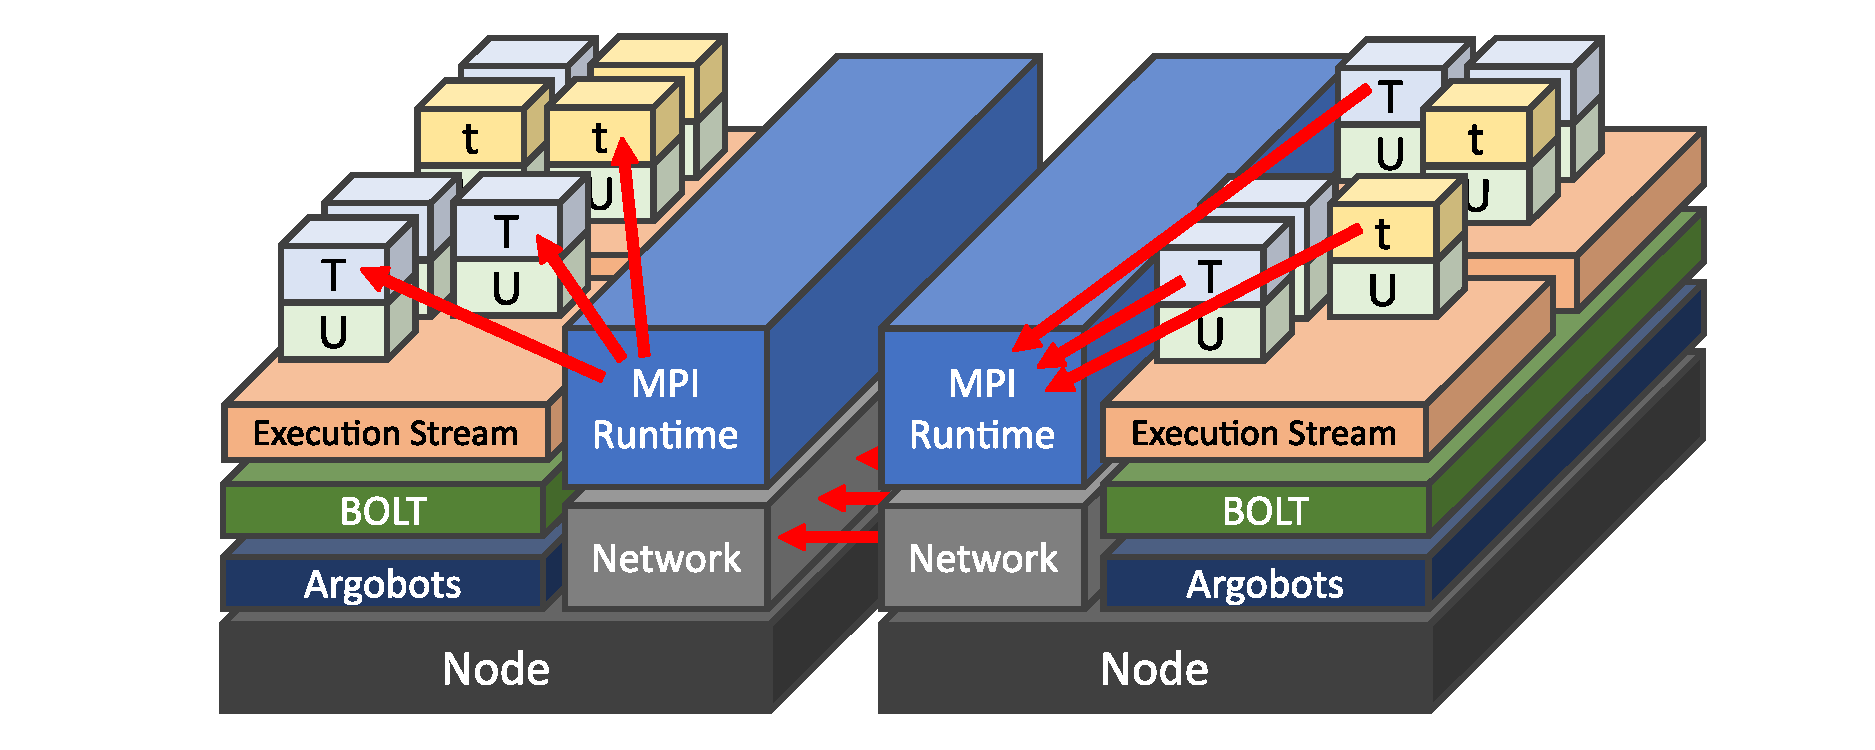
\includegraphics[width=0.9\columnwidth]{projects/2.3.2-Tools/2.3.2.11-SOLLVE/SOLLVE-BOLT.pdf}

  \caption{\label{fig:sollve-bolt} MPI+Threads interoperability of
  BOLT.  OpenMP threads and tasks in BOLT interact MPI implementations
  via the Argobots layer.}
\end{figure}

We improved the interoperability of BOLT with various MPI systems via
lightweight threads, Argobots.  Since most MPI runtimes including
MPICH, Open~MPI, and production MPI implementations that are derived
from either MPICH or Open~MPI assume OS-level threads as ``Thread'' in
MPI+Thread, lightweight OpenMP runtimes based on lightweight threads
failed to interoperate well with existing MPI systems.  To address
this issue, we have implemented an abstracted threading layer for
lightweight threads in these MPI runtimes so that users can choose
OpenMP threads and tasks of BOLT as ``Thread''.

Virtual communication interfaces (VCIs) in MPICH are mapped to logically parallel MPI operations, can benefit both multi-thread and multi-GPU configurations since both rely on VCIs for parallel communication. We developed VCI-aware OpenMP thread scheduling over BOLT via a user-level threading interoperability layer significantly reduces the locking overheads, realizing highly scalable MPI communication. The evaluation using ORNL Spock (Slingshot) shows significant performance improvement.

Our latest BOLT 1.0 release contains a large upgrade to be compatible
with LLVM OpenMP 10.0, which further improves performance and
functionalities especially for GPU offloading and new OpenMP 5.0
features.  This release also contains scheduler improvement in BOLT
and an upgrade of the Argobots package, which allows further
lightweight fine-grained OpenMP threading and tasking.  Interaction
and integration are a critical piece for the BOLT project.  We
continue working on the SOLLVE Spack package so that this BOLT system
is available on our target HPC systems and users can utilize BOLT for
(1) ECP applications that have fine-grained parallelism such as nested
parallel regions and tasking (e.g., ECP SLATE) and (2) runtime systems
via the Argobots layer (such as MPICH and Open MPI we mentioned) that
can take advantage of ULT's lightweight synchronization for resource
management.

\paragraph{Next Steps}

One of the largest advantages of BOLT is an underlying lightweight
thread implementation, flexible scheduling, and high interoperability
thanks to Argobots. The following list includes our next plans:

\begin{enumerate}

\item Explores opportunities for utilizing lightweight threads for
other optimizations in the context of OpenMP.  The main focus of BOLT
has been the performance of fine-grained OpenMP threads, so we have
not fully explored how BOLT could elevate the performance of other
parallel units (e.g., data-dependent tasking and GPU offloading). We
are planning to investigate room for optimizations and implement them
with evaluation.

\item Investigates the performance with large-scale applications.
In order to find potential room for optimizations and evaluate the
performance of BOLT in real large-scale workloads, we further
investigate other SOLLVE components and ECP applications that can benefit from BOLT.  Since most distributed systems rely on MPI for internode
communication, we will also work on tighter integration with MPI to
optimize the performance with MPI runtimes over BOLT.

\end{enumerate}
